\documentclass[tikz]{standalone}
\usetikzlibrary{arrows.meta}
\begin{document}

\begin{tikzpicture}[rotate=180,-latex, arrows={Triangle[angle=20:5pt,scale=1.5]-}]
	\node (A1) at (0,-3) {\(A\)};
	\node (A2) at (3,0) {\(A\)};
	\node (B) at (3,-3) {\(B\)};
	\node (C) at (0,0) {\(C\)};

	\draw (C) to node [below] {\(q\)} (A2);
	\draw (C) to node [right] {\(q\)} (A1);
	\draw (A1) to node [above] {\(f\)} (B);
	\draw (A2) to node [left] {\(g\)} (B);
\end{tikzpicture}

\begin{tikzpicture}[rotate=180,-latex, arrows={Triangle[angle=20:5pt,scale=1.5]-}]
	\node (A1) at (0,-3) {\(A\)};
	\node (A2) at (3,0) {\(A\)};
	\node (B) at (3,-3) {\(B\)};
	\node (D) at (0,0) {\(D\)};

	\draw (D) to node [below] {\(h\)} (A2);
	\draw (D) to node [right]  {\(h\)} (A1);
	\draw (A1) to node [above] {\(f\)} (B);
	\draw (A2) to node [left] {\(g\)} (B);
\end{tikzpicture}

\begin{tikzpicture}[rotate=180,-latex, arrows={Triangle[angle=20:5pt,scale=1.5]-}]
	\node (C) at (0,0) {\(C\)};
	\node (D) at (0,3) {\(D\)};
	\node (A) at (3,0) {\(A\)};

	\draw (C) to node [above] {\(q\)} (A);
	\draw (D) to node [right] {\(k\)} (C);
	\draw (D) to node [below left] {\(h\)} (A);
\end{tikzpicture}

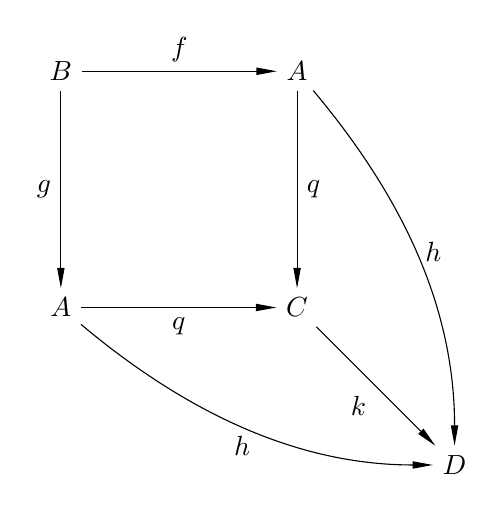
\begin{tikzpicture}[rotate=180,-latex, arrows={Triangle[angle=20:5pt,scale=1.5]-}]
	\node (A1) at (0,-3) {\(A\)};
	\node (A2) at (3,0) {\(A\)};
	\node (B) at (3,-3) {\(B\)};
	\node (C) at (0,0) {\(C\)};
	\node (D) at (-2,2) {\(D\)};

	\draw (C) to node [below] {\(q\)} (A2);
	\draw (C) to node [right] {\(q\)} (A1);
	\draw (A1) to node [above] {\(f\)} (B);
	\draw (A2) to node [left] {\(g\)} (B);

	\draw (D) to node [below left] {\(k\)} (C);
	\draw (D) to [out=-90 , in=130] node [right] {\(h\)} (A1);
	\draw (D) to [out=0 , in=140] node [below] {\(h\)} (A2);
\end{tikzpicture}

\end{document}
